% Hopper — Software Design Document (SDD)
% CSE 4113: Internet Programming Lab — course submission (standalone PDF; compile with pdflatex x2)

\documentclass[12pt,a4paper]{article}

\usepackage[margin=2.5cm]{geometry}
\setlength{\headheight}{14pt}
\usepackage[T1]{fontenc}
\usepackage[utf8]{inputenc}
\usepackage{newtxtext,newtxmath}
\usepackage{microtype}
\usepackage{setspace}
\usepackage{titlesec}
\usepackage{fancyhdr}
\usepackage[dvipsnames,table]{xcolor}
\usepackage{booktabs}
\usepackage{longtable}
\usepackage{tabularx}
\usepackage{array}
\usepackage{multirow}
\usepackage{enumitem}
\usepackage{hyperref}
\usepackage{graphicx}
\usepackage{float}
\usepackage{caption}
\usepackage{amsmath}
\usepackage{tikz}
\usetikzlibrary{arrows.meta,calc,positioning}
\usepackage{parskip}

%% Hyperref
\hypersetup{
  colorlinks   = true,
  linkcolor    = RoyalBlue,
  urlcolor     = RoyalBlue,
  citecolor    = RoyalBlue,
  pdftitle     = {Hopper -- Software Design Document},
  pdfauthor    = {Hopper Project Teams},
  bookmarksnumbered = true,
  bookmarksopen     = true,
}

%% Section titles
\titleformat{\section}{\large\bfseries\color{RoyalBlue}}{\thesection}{0.75em}{}
\titleformat{\subsection}{\normalsize\bfseries}{\thesubsection}{0.65em}{}
\titleformat{\subsubsection}{\normalsize\itshape}{\thesubsubsection}{0.55em}{}

%% Header / footer
\pagestyle{fancy}
\fancyhf{}
\fancyhead[L]{\small\textit{Hopper (Hopper Cloud) --- Software Design Document v0.1}}
\fancyhead[R]{\small\textit{CSE 4113}}
\fancyfoot[C]{\small Page \thepage}
\renewcommand{\headrulewidth}{0.4pt}
\renewcommand{\footrulewidth}{0pt}

%% Table helpers
\newcolumntype{L}[1]{>{\raggedright\arraybackslash}p{#1}}
\newcolumntype{C}[1]{>{\centering\arraybackslash}p{#1}}
\newcolumntype{R}[1]{>{\raggedleft\arraybackslash}p{#1}}
\renewcommand{\arraystretch}{1.28}

%% Team names: use \ByteMe in body text next to \textbf{Four-Eyed Raven}; use \ByteMeHeading where bold is already set (e.g.\ subsubsection titles are italic, not bold)
\newcommand{\ByteMeHeading}{Byte Me}
\newcommand{\ByteMe}{%
  \texorpdfstring{\textbf{\ByteMeHeading}}{Byte Me}%
}
\begin{document}

% ── Title page ───────────────────────────────────────────────────────────────
\begin{titlepage}
  \centering
  \vspace*{1cm}
  {\Large\textbf{CSE 4113: Internet Programming Lab}\par}
  \vspace{0.75cm}
  {\huge\textbf{\textcolor{RoyalBlue}{Software Design Document}}\par}
  \vspace{0.35cm}
  {\LARGE\textbf{Hopper (Hopper Cloud)}\par}
  \vspace{0.25cm}
  {\large\itshape A VM / compute provisioning panel for universities\par}
  \vspace{1.5cm}

  \begin{tabular}{@{}ll@{}}
    \textbf{Deliverable:} & Software Design Document (SDD) \\
    \textbf{Document version:} & 0.2 \\
    \textbf{Date:} & April 2026 \\
    \textbf{Repository:} & \url{https://github.com/CREVIOS/Hopper} \\
  \end{tabular}

  \vspace{1.25cm}
  {\large\textbf{Submitted to}\par}
  \vspace{0.4cm}
  \textit{Prof.\ Dr.\ Md.\ Mamun Or Rashid}\\
  \textit{Mr.\ Md.\ Fahim Arefin}\\
  \textit{Mr.\ Md.\ Ahasanul Alam}

  \vfill
  \begin{minipage}{0.92\textwidth}
    \small
    \textbf{Collaborating teams:} \textbf{Four-Eyed Raven} (Team~1) and \ByteMe{} (Team~2) jointly contribute to this project; the design below merges both teams' requirements into a single shared system.\\
    Related requirement documents are summarized in Section~\ref{sec:references} and Appendix~\ref{app:alignment}.
  \end{minipage}
  \vspace{0.75cm}
\end{titlepage}

\setcounter{page}{1}

\begin{abstract}
\noindent
This Software Design Document specifies the \textbf{architecture and major design decisions} for \textbf{Hopper}, a self-hosted platform that gives students and staff \textbf{self-service access} to isolated workloads on \textbf{Kubernetes}, with \textbf{institutional SSO (Keycloak)}, \textbf{credit-based usage}, and a \textbf{web portal (SvelteKit)} backed by a \textbf{FastAPI} gateway and a \textbf{Go} orchestration service. The design reflects a \textbf{collaboration} between \textbf{Four-Eyed Raven} and \ByteMe{}, bringing together both teams' Software Requirements Specifications into one consolidated implementation.
\end{abstract}

\tableofcontents
\newpage

% ═══════════════════════════════════════════════════════════════════════════
\section{Document control}
\label{sec:doc-control}

\begin{tabularx}{\textwidth}{@{}L{3.2cm}X@{}}
  \toprule
  \textbf{Field} & \textbf{Value} \\
  \midrule
  Course & CSE 4113: Internet Programming Lab \\
  Deliverable & Software Design Document (SDD) \\
  Project & Hopper (Hopper Cloud) --- a VM / compute provisioning panel for universities \\
  Submitted to & Prof.\ Dr.\ Md.\ Mamun Or Rashid; Mr.\ Md.\ Fahim Arefin; Mr.\ Md.\ Ahasanul Alam \\
  Document version & 0.2 \\
  Date & April 2026 \\
  \bottomrule
\end{tabularx}

\subsection{Authorship and team structure}
\textbf{Collaboration model:} \textbf{Four-Eyed Raven} (Team~1) and \ByteMe{} (Team~2) work as \textbf{partners} on one product: both teams shape requirements and implementation toward a \textbf{single} product and roadmap. The Four-Eyed Raven SRS emphasizes GPU-centric cloud and institutional controls; the \ByteMe{} SRS adds VM lifecycle, approvals, quotas, and related workflows---together they inform a \textbf{unified} Hopper design rather than separate products.

\subsection{Authors by team}

\subsubsection*{Four-Eyed Raven (Team~1)}
\begin{tabularx}{\textwidth}{@{}L{4.5cm}X@{}}
  \toprule
  \textbf{Name} & \textbf{Identifier / contact} \\
  \midrule
  Tazkia Malik & Roll 7 --- \texttt{maliktazkia@gmail.com} \\
  Md.\ Sadek Hossain Asif & Roll 15 --- \texttt{asifsadek509@gmail.com} \\
  Tanzila Khan & Roll 25 --- \texttt{tanzila011001@gmail.com} \\
  Taif Ahmed Turjo & Roll 45 --- \texttt{ahmedtaif437@gmail.com} \\
  \bottomrule
\end{tabularx}

\subsubsection*{\ByteMeHeading{} (Team~2)}
\begin{tabularx}{\textwidth}{@{}L{4.5cm}X@{}}
  \toprule
  \textbf{Name} & \textbf{Identifier / contact} \\
  \midrule
  Anindya Kundu & Roll 09 --- \texttt{sanindya50@gmail.com} \\
  Kabya Mithun Saha & Roll 16 --- \texttt{kabyasaha1812@gmail.com} \\
  Md.\ Muhaiminul Islam Ninad & Roll 43 --- \texttt{ninadgns@gmail.com} \\
  Fayek Ahmed & Roll 57 --- \texttt{fayekahmedrahat90@gmail.com} \\
  \bottomrule
\end{tabularx}

\subsection{Revision history}
\begin{tabularx}{\textwidth}{@{}c L{2.2cm} X@{}}
  \toprule
  \textbf{Version} & \textbf{Date} & \textbf{Summary} \\
  \midrule
  0.1 & April 2026 & Initial SDD: unified design merging both teams' SRS themes \\
  0.2 & April 2026 & Traceability, interface/event specs, flows, state machines, data/security/NFR/deployment/config/testing depth, glossary \\
  \bottomrule
\end{tabularx}

% ═══════════════════════════════════════════════════════════════════════════
\section{Purpose and scope of this SDD}
\label{sec:purpose}

\subsection{Purpose}
\begin{itemize}[leftmargin=*]
  \item Record \textbf{what} the system does at a design level (major components, data, interfaces, security boundaries).
  \item Give \textbf{all eight members} a single reference for how work maps to architecture.
  \item Document how \textbf{Four-Eyed Raven} and \ByteMe{} SRS themes relate to a single implementation (see \S\ref{sec:doc-control} and Section~\ref{sec:context}).
\end{itemize}

\subsection{In scope (design)}
Web portal, API gateway, orchestration service, persistence, eventing, and Kubernetes integration as implemented or specified for the product. Cross-cutting concerns: authentication, credits/ledger, session/pod lifecycle, observability hooks.

\subsection{Out of scope (this document)}
Low-level line-by-line API listing (refer to the API gateway's OpenAPI/Swagger documentation when running). Full hypervisor/vSphere/Proxmox integration (\ByteMe{} SRS assumed external APIs; Hopper targets Kubernetes---see \S\ref{sec:srs-k8s-alignment}).

% ═══════════════════════════════════════════════════════════════════════════
\section{System context}
\label{sec:context}

\subsection{Problem summary (by team, merged product)}
\begin{itemize}[leftmargin=*]
  \item \textbf{Four-Eyed Raven --- Hopper Cloud:} Students need \textbf{fair, isolated access} to institutional \textbf{GPU} (and related) compute without ad-hoc admin work; \textbf{credits}, \textbf{auditability}, \textbf{gVisor}, \textbf{network policy}, and \textbf{Teleport-class SSH} are central.
  \item \textbf{\ByteMe{} --- VMpire:} Academic \textbf{VM} provisioning suffers from \textbf{manual approvals}, \textbf{weak quota enforcement}, and \textbf{poor lifecycle visibility}; emphasis on \textbf{approval queues}, \textbf{per-role dashboards}, \textbf{expiration policies}, and \textbf{notifications}.
\end{itemize}

\textbf{Unified stance:} The \textbf{shipping system} is \textbf{Hopper} on \textbf{Kubernetes}: user-facing ``VMs'' are \textbf{workload sessions backed by Pods}, with plan tiers and orchestration mapping user-visible SKUs to cluster resources. \textbf{GPU} depth is specified in the Four-Eyed Raven SRS; some deployments may emphasize CPU/RAM tiers first while the design evolves---throughout, \textbf{orchestrator + plans} remain the abstraction for tiered compute.

\subsection{Stakeholders (combined)}
Students/researchers, lab administrators, instructors/PIs, platform engineers, and institutional IT---as in both SRS documents---with \textbf{role models} converging toward: student, TA, professor, department admin, university admin, platform admin, together with \textbf{instructor} and \textbf{lab admin} dashboard needs from the combined requirements set (some items remain \textbf{backlog} features to schedule in later milestones).

% ═══════════════════════════════════════════════════════════════════════════
\section{Design goals and constraints}
\label{sec:goals}

\begin{tabularx}{\textwidth}{@{}L{4.2cm} X@{}}
  \toprule
  \textbf{Goal} & \textbf{Design implication} \\
  \midrule
  Security-first multi-tenancy & Default-deny networking (Calico/Cilium per deployment), curated images, identity via Keycloak \\
  Fair usage & Double-entry \textbf{credit ledger}, per-minute metering, automated termination on exhaustion \\
  Operational simplicity & Few moving parts at app layer: FastAPI + Go orchestrator + Postgres + NATS \\
  Academic SSO & OIDC through Keycloak; SAML brokering as per deployment docs \\
  Four-Eyed Raven non-goals & No public multi-tenant SaaS, no real-money payments in v1, no student-built image registry in v1 \\
  Lifecycle \& admin themes & \textbf{Approval-before-provision}, \textbf{richer expiration notifications}, \textbf{course-scoped quotas} $\rightarrow$ \textbf{coordinated} with the shared architecture (see Section~\ref{sec:flows}; roadmap Section~\ref{sec:roadmap}) \\
  \bottomrule
\end{tabularx}

\vspace{0.5em}
\noindent\textbf{Technical constraints} (from the SRS documents and implementation): PostgreSQL with relational schema migrations; gRPC between API gateway and orchestrator; NATS JetStream for billing/metrics events; Kubernetes API for workload lifecycle.

% ═══════════════════════════════════════════════════════════════════════════
\section{High-level architecture}
\label{sec:architecture}

The runtime architecture is summarized below (consistent with Sections~\ref{sec:components}--\ref{sec:flows}).

\begin{center}
\resizebox{0.99\linewidth}{!}{%
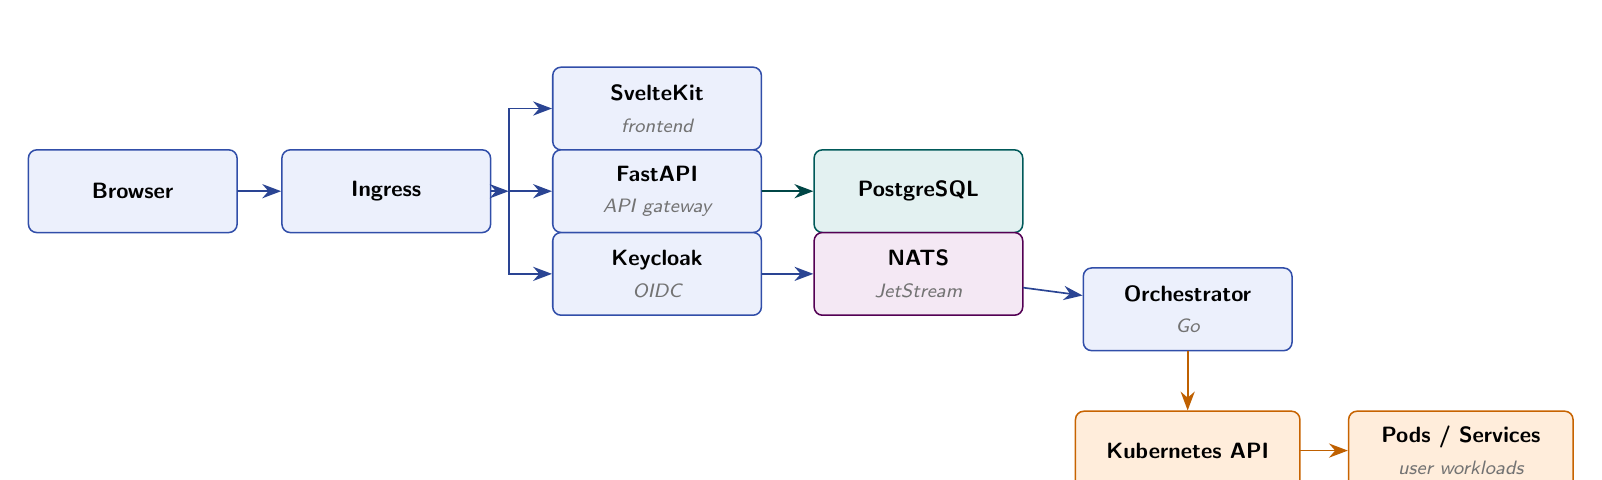
\begin{tikzpicture}[
  font=\sffamily\footnotesize,
  >={Stealth[length=2.4mm]},
  line cap=round,
  arrA/.style={-{Stealth[length=2.4mm]}, semithick, draw=RoyalBlue!65!black},
  arrD/.style={-{Stealth[length=2.4mm]}, semithick, draw=teal!55!black},
  arrP/.style={-{Stealth[length=2.4mm]}, semithick, draw=orange!75!black},
  app/.style={rectangle, rounded corners=3pt, minimum width=2.65cm, minimum height=1.05cm,
    inner sep=4pt, align=center, draw=RoyalBlue!75!black, line width=0.55pt, fill=RoyalBlue!10},
  data/.style={app, draw=teal!70!black, fill=teal!11},
  msg/.style={app, draw=violet!65!black, fill=violet!9},
  plat/.style={rectangle, rounded corners=3pt, minimum width=2.85cm, minimum height=1.0cm,
    inner sep=4pt, align=center, draw=orange!78!black, line width=0.55pt, fill=orange!14},
]
  % Access + app tier (left to mid)
  \node[app] (browser) at (0,0) {\textbf{Browser}};
  \node[app, right=0.55cm of browser] (ingress) {\textbf{Ingress}};
  \coordinate (fork) at ($(ingress.east)+(0.22,0)$);
  \node[app, anchor=west] (svelte) at ($(fork)+(0.55,1.05)$)
    {\textbf{SvelteKit}\\[2pt]{\scriptsize\itshape\color{black!55}frontend}};
  \node[app, anchor=west] (gw) at ($(fork)+(0.55,0)$)
    {\textbf{FastAPI}\\[2pt]{\scriptsize\itshape\color{black!55}API gateway}};
  \node[app, anchor=west] (kc) at ($(fork)+(0.55,-1.05)$)
    {\textbf{Keycloak}\\[2pt]{\scriptsize\itshape\color{black!55}OIDC}};
  % Data + messaging
  \node[data, right=0.65cm of gw] (pg) {\textbf{PostgreSQL}};
  \node[msg, right=0.65cm of kc] (nats) {\textbf{NATS}\\[2pt]{\scriptsize\itshape\color{black!55}JetStream}};
  % Orchestrator sits on the event path from NATS
  \node[app, anchor=west] (orch) at ($(nats.east)+(0.75,-0.45)$)
    {\textbf{Orchestrator}\\[2pt]{\scriptsize\itshape\color{black!55}Go}};
  % Platform
  \node[plat, below=0.75cm of orch] (kapi) {\textbf{Kubernetes API}};
  \node[plat, right=0.6cm of kapi] (pods) {\textbf{Pods / Services}\\[2pt]{\scriptsize\itshape\color{black!55}user workloads}};
  % Arrows: browser chain
  \draw[arrA] (browser) -- (ingress);
  \draw[arrA] (ingress.east) -- (fork);
  \draw[arrA] (fork) |- (svelte.west);
  \draw[arrA] (fork) -- (gw.west);
  \draw[arrA] (fork) |- (kc.west);
  \draw[arrD] (gw) -- (pg);
  \draw[arrA] (kc) -- (nats);
  \draw[arrA] (nats) -- (orch);
  \draw[arrP] (orch) -- (kapi);
  \draw[arrP] (kapi) -- (pods);
\end{tikzpicture}%
}
\end{center}

\textbf{Layers:}
\begin{enumerate}[leftmargin=*]
  \item \textbf{Access:} Keycloak (auth); SSH via NodePort in simpler deployments, or Teleport-class access where integrated.
  \item \textbf{Application:} SvelteKit UI; FastAPI REST + SSE; Go orchestrator (gRPC server, billing ticker, K8s integration, NATS publish).
  \item \textbf{Data:} PostgreSQL (users, sessions, append-only ledger); optional TimescaleDB for metrics time-series as deployed.
  \item \textbf{Platform:} Kubernetes cluster, GPU/CPU scheduling stack, network policies, and GPU Operator (or equivalent) as configured per environment.
\end{enumerate}

% ═══════════════════════════════════════════════════════════════════════════
\section{Component design}
\label{sec:components}

\subsection{Web frontend (SvelteKit)}
\begin{itemize}[leftmargin=*]
  \item \textbf{SvelteKit 2 / Svelte 5} with server loads and client stores (e.g.\ auth and pod state).
  \item \textbf{Routes:} dashboard, pods (list + detail with metrics/terminal placeholders), credits, admin stub, login.
  \item \textbf{Transport:} HTTP to \texttt{/api}; SSE for pod metrics where implemented.
\end{itemize}
\textbf{Design note:} Some dashboard features described in the SRS documents (for example approval queues, a global workload table, and quota panels) are \textbf{not yet fully implemented} in the baseline; they are \textbf{scheduled} for future milestones (see roadmap Section~\ref{sec:roadmap}).

\subsection{API gateway (FastAPI)}
\begin{itemize}[leftmargin=*]
  \item \textbf{FastAPI} application: routers for \texttt{auth}, \texttt{pods}, \texttt{credits}, \texttt{admin}.
  \item \textbf{Responsibilities:} OIDC session handling, JWT validation, credit checks on create, ledger operations, NATS consumption for billing deductions, SSE bridging for metrics.
  \item \textbf{Persistence:} SQLAlchemy async models: \texttt{User}, \texttt{Account}, \texttt{Transfer}, \texttt{LedgerEntry}, \texttt{PodSession} (relational migrations).
\end{itemize}

\subsection{Orchestrator (Go)}
\begin{itemize}[leftmargin=*]
  \item \textbf{Go} service: gRPC \textbf{Pod} and \textbf{Billing} services, K8s client, NATS publishers, periodic billing/metrics loops (internal packages for gRPC, Kubernetes, pod lifecycle, billing, events).
  \item \textbf{Responsibilities:} Create/terminate pods, reflect status, stream metrics to gateway path, emit billing events.
\end{itemize}

\subsection{SRS alignment with the Kubernetes implementation}
\label{sec:srs-k8s-alignment}
Hopper is built around \textbf{one} runtime: the \textbf{Kubernetes API} plus the gateway and orchestrator described above. Both teams' SRS documents are read against that shared center of gravity; this subsection records \emph{where} each document already matches the implementation and \emph{where} wording in an SRS assumed something else.

\subsubsection*{Four-Eyed Raven (Hopper Cloud)}
The Hopper Cloud baseline (GPU-centric workloads, credits, isolation, institutional SSO, network policy, observability hooks) is expressed in terms of \textbf{pods}, \textbf{scheduling}, and \textbf{cluster policy}---the same primitives this SDD's components implement. The product name in the SRS (\textbf{Hopper}) matches the orchestration model described in \S\ref{sec:architecture}--\ref{sec:components}; no extra indirection layer is required to relate that SRS to this design.

\subsubsection*{\ByteMe{} (VMpire)}
The VMpire SRS describes provisioning via a \textbf{hypervisor REST API} (e.g.\ vSphere/Proxmox-style surfaces). \textbf{Hopper standardizes on Kubernetes}: concrete provisioning is \textbf{namespace/pod/service} creation, not a second hypervisor backend. Workflow ideas such as \textbf{pending $\rightarrow$ approved $\rightarrow$ provisioning} are realized as \textbf{workflow state} and \textbf{admin APIs} on the same orchestrator and database, not a parallel provisioning stack.

\subsection{Protocol contracts (gRPC / Protocol Buffers)}
\begin{itemize}[leftmargin=*]
  \item Package \texttt{hopper/pod/v1} --- \texttt{PodOrchestrator}: create, terminate, status, metrics stream, etc.
  \item Package \texttt{hopper/billing/v1} --- \texttt{BillingService}: deduct, balance, usage stream.
\end{itemize}
Contract types are generated from these definitions in the normal project build (container or local toolchain).

\subsection{Infrastructure and deployment automation}
\begin{itemize}[leftmargin=*]
  \item \textbf{Pulumi} (Python) and \textbf{Ansible} playbooks for bring-up.
  \item \textbf{Kubernetes manifests} for deployables, network policies, and scheduler/GPU operator configuration as appropriate per environment.
  \item \textbf{Observability} stack configs (Prometheus, Grafana, Loki) shipped with the deployment.
\end{itemize}
REST/gRPC/NATS/SSE surfaces and state machines: Appendix~\ref{app:interfaces}, Appendix~\ref{app:state-machines}.

% ═══════════════════════════════════════════════════════════════════════════
\section{Data design}
\label{sec:data}

\subsection{Core entities (as implemented)}
\begin{itemize}[leftmargin=*]
  \item \textbf{User} --- identity, role, university linkage.
  \item \textbf{Account / Transfer / LedgerEntry} --- double-entry credit ledger; immutability enforced at DB layer (rules/triggers per migrations).
  \item \textbf{PodSession} --- session lifecycle, plan/tier fields, SSH metadata, status, charges.
\end{itemize}

\subsection{\ByteMe{} data concepts (future alignment)}
Entities from the \ByteMe{} VMpire SRS---\textbf{VM Request}, \textbf{Quota Policy} scoped by course/department, \textbf{Notification}---should be introduced \textbf{without breaking} ledger integrity: e.g.\ \texttt{vm\_requests} or \texttt{provisioning\_requests} table with FK to \texttt{users}, state machine \textbf{pending $\rightarrow$ approved $\rightarrow$ \ldots} joining to \texttt{PodSession} on approval.

Relationships, indexes, ledger locking: Appendix~\ref{app:data-depth}.

% ═══════════════════════════════════════════════════════════════════════════
\section{Key runtime flows}
\label{sec:flows}

\subsection{Create session (``VM'')}
\begin{enumerate}[leftmargin=*]
  \item User selects \textbf{plan/tier} $\rightarrow$ \texttt{POST /pods/} with auth cookie.
  \item Gateway validates JWT, checks \textbf{credit sufficiency}, creates \textbf{PodSession}, calls orchestrator \textbf{CreatePod} via gRPC.
  \item Orchestrator creates K8s resources; returns connection info (e.g.\ SSH port).
  \item \textbf{Billing loop:} orchestrator ticks $\rightarrow$ NATS \texttt{billing.deducted} $\rightarrow$ gateway updates ledger; on zero balance, exhaustion path triggers termination.
\end{enumerate}

\subsection{Terminate session}
User or admin triggers delete $\rightarrow$ gateway $\rightarrow$ orchestrator \textbf{TerminatePod} $\rightarrow$ cleanup; ledger and session state updated; events emitted.

\subsection{Observability path}
Metrics from orchestrator $\rightarrow$ NATS / SSE $\rightarrow$ dashboard components (\texttt{GpuMetrics} / CPU-RAM analogs depending on build).

Failure branches, idempotency, and ordering: Appendix~\ref{app:critical-flows}.

% ═══════════════════════════════════════════════════════════════════════════
\section{Security design}
\label{sec:security}

\begin{tabularx}{\textwidth}{@{}L{3.5cm} X@{}}
  \toprule
  \textbf{Concern} & \textbf{Approach} \\
  \midrule
  Authentication & Keycloak OIDC; JWT validation in gateway \\
  Authorization & Role claims; route guards server-side \\
  Network & Default-deny policies; documented Cilium/Calico intent \\
  Audit & Ledger + session events; expand to full audit table per Four-Eyed Raven FR-HC-21 and \ByteMe{} FR-AUDIT-001 \\
  Isolation & gVisor/runtime class and policies per deployment hardening for GPU rollout \\
  \bottomrule
\end{tabularx}

\vspace{0.5em}
\noindent Extended: threat model, secrets, token lifetimes, and trust boundaries are in Appendix~\ref{app:security-extended}.

% ═══════════════════════════════════════════════════════════════════════════
\section{Non-functional design}
\label{sec:nfr}

\begin{tabularx}{\textwidth}{@{}L{3.8cm} X@{}}
  \toprule
  \textbf{Area} & \textbf{Target (from combined SRS and this SDD)} \\
  \midrule
  Availability & Health endpoints; K8s replicas for stateless tiers \\
  Performance & API responsiveness for dashboard; SSE for metrics; orchestrator tick interval documented \\
  Observability & Prometheus/Grafana/Loki stack; structured logging in gateway \\
  Testing & Unit, integration, end-to-end, and load tests as automated in the project \\
  \bottomrule
\end{tabularx}

\vspace{0.5em}
\noindent Measurable targets, backup/RPO/RTO, and ``TBD'' placeholders are consolidated in Appendix~\ref{app:nfr-targets} with SRS NFR IDs.

% ═══════════════════════════════════════════════════════════════════════════
\section{Evolution roadmap (design-level)}
\label{sec:roadmap}

\begin{tabularx}{\textwidth}{@{}L{3cm} X@{}}
  \toprule
  \textbf{Phase} & \textbf{Emphasis} \\
  \midrule
  \textbf{Current} & MVP: SSO, pod/session lifecycle, credits, admin stubs, K8s deployment \\
  \textbf{Next} & \textbf{Together:} platform hardening (RBAC depth, audit log UI, Teleport/gVisor/GPU operator as environments mature) \textbf{and} collaborative features from the combined SRS (approval workflow, quotas, notifications, instructor/lab dashboards) \\
  \textbf{Later} & Full GPU tier UX parity with the design goals above; optional external hypervisor only if an institution requires non-K8s assets \\
  \bottomrule
\end{tabularx}

% ═══════════════════════════════════════════════════════════════════════════

\newpage
\section{References}
\label{sec:references}

\begin{itemize}[leftmargin=*]
  \item \textbf{Software Requirements Specifications} (companion deliverables, cited by ID throughout this SDD): \emph{Hopper Combined SRS} (v0.1); \emph{Four-Eyed Raven / Hopper Cloud SRS}; \emph{\ByteMeHeading{} (VMpire) SRS}.
  \item \textbf{Interface contracts:} gRPC services and messages defined in the \texttt{hopper/} Protocol Buffer packages (pod and billing); HTTP API described by the API gateway's OpenAPI schema (interactive \texttt{/docs} when the gateway is running).
  \item \textbf{Further reading} (optional, for operators): vendor and security advisories referenced by the deployment (e.g.\ GPU scheduling, relevant CVEs) are maintained with the deployment materials, not duplicated here.
\end{itemize}

% ═══════════════════════════════════════════════════════════════════════════
\appendix

\section{Requirements traceability}
\label{app:traceability}

Maps SRS requirement IDs to this SDD and to the \textbf{primary component or area} in the implementation. ``Partial / backlog'' means not fully implemented or only partially aligned.

\subsection{Four-Eyed Raven SRS --- functional}

{\small
\begin{longtable}{@{}p{2.4cm} p{2.8cm} p{4.2cm} p{4.8cm}@{}}
  \toprule
  \textbf{ID} & \textbf{SDD section(s)} & \textbf{Primary component / area} & \textbf{Notes} \\
  \midrule
  \endfirsthead
  \multicolumn{4}{c}{\tablename\ \thetable{} --- \textit{continued}} \\
  \toprule
  \textbf{ID} & \textbf{SDD section(s)} & \textbf{Primary component / area} & \textbf{Notes} \\
  \midrule
  \endhead
  \midrule
  \multicolumn{4}{r}{\textit{Continued on next page}} \\
  \endfoot
  \bottomrule
  \endlastfoot
  FR-HC-01, FR-HC-02 & \S\ref{sec:architecture}--\ref{sec:components}, \S\ref{sec:security}, App.~\ref{app:interfaces} & API gateway auth router and session/JWT middleware & OIDC; token expiry $\rightarrow$ 401 \\
  FR-HC-03--05 & \S\ref{sec:components}--\ref{sec:data}, App.~\ref{app:data-depth} & Credits router, credit service, ledger models, DB migrations & Ledger + DB rules \\
  FR-HC-06--08, FR-HC-25 & \S\ref{sec:components}--\ref{sec:flows}, App.~\ref{app:critical-flows}--\ref{app:state-machines} & Pods router; web UI pod routes & Create/list/terminate \\
  FR-HC-09--11, FR-HC-24 & \S\ref{sec:architecture}--\ref{sec:components} & Cluster manifests; orchestrator Kubernetes client & GPU/MIG/time-slice: env-dependent \\
  FR-HC-12--13 & \S\ref{sec:architecture} & SSH exposure (NodePort POC; Teleport-class access TBD) & NodePort SSH in POC \\
  FR-HC-14--15 & \S\ref{sec:architecture}, App.~\ref{app:security-extended} & Kubernetes NetworkPolicies & Calico/Cilium as deployed \\
  FR-HC-16--18 & \S\ref{sec:flows}, App.~\ref{app:critical-flows} & Gateway billing NATS consumer; orchestrator ticker & Reaper = exhaust path + TTL backlog \\
  FR-HC-19--20 & \S\ref{sec:components} & Credits and admin routers & Admin UI partial \\
  FR-HC-21 & \S\ref{sec:data}, App.~\ref{app:data-depth} & Audit table: backlog; ledger is audit-like & \\
  FR-HC-22--23 & \S\ref{sec:components} & PVC / storage strategy vs cluster deployment & \\
  FR-HC-26 & App.~\ref{app:interfaces} & Auth routes (logout) & \\
  FR-HC-27 & --- & Partial / backlog & Session extend \\
\end{longtable}
}

\subsection{Four-Eyed Raven --- non-functional}
\begin{tabularx}{\textwidth}{@{}p{2.5cm} p{3cm} X@{}}
  \toprule
  \textbf{ID} & \textbf{SDD / appendix} & \textbf{Evidence / note} \\
  \midrule
  NFR-HC-1--4 & App.~\ref{app:nfr-targets} & Latencies: provisioning timeout 30s gRPC client; billing 1 min tick \\
  NFR-HC-5--18 & App.~\ref{app:nfr-targets}, \ref{app:deployment} & HA, mTLS, gVisor, observability: partial vs full hardening targets \\
  NFR-HC-10 & App.~\ref{app:critical-flows}, \ref{app:data-depth} & Idempotency keys: \textbf{not} implemented for NATS deductions; ledger uses DB transaction + advisory lock \\
  \bottomrule
\end{tabularx}

\subsection{\ByteMe{} (VMpire) SRS --- functional}

{\small
\begin{longtable}{@{}p{2.4cm} p{2.8cm} p{4cm} p{5cm}@{}}
  \toprule
  \textbf{ID} & \textbf{SDD section(s)} & \textbf{Primary component / area} & \textbf{Notes} \\
  \midrule
  \endfirsthead
  \multicolumn{4}{c}{\tablename\ \thetable{} --- \textit{continued}} \\
  \toprule
  \textbf{ID} & \textbf{SDD section(s)} & \textbf{Primary component / area} & \textbf{Notes} \\
  \midrule
  \endhead
  \midrule
  \multicolumn{4}{r}{\textit{Continued on next page}} \\
  \endfoot
  \bottomrule
  \endlastfoot
  FR-REQ-001, FR-REQ-002 & \S\ref{sec:srs-k8s-alignment}, \S\ref{sec:data} & Backlog --- no approval queue table/API yet & Workflow future \\
  FR-QUOTA-001, FR-QUOTA-002 & \S\ref{sec:goals} & Partial: credits + max 3 concurrent sessions (pods router) & Course quotas backlog \\
  FR-MON-001--003 & \S\ref{sec:components}, App.~\ref{app:interfaces} & Dashboard + admin stub; metrics SSE & Global admin VM view partial \\
  FR-LIFE-001--003 & App.~\ref{app:state-machines} & \texttt{PodSession.state} simpler than Expiring$\rightarrow$Decommissioned & Align over time \\
  FR-REQ-003 & --- & Backlog & Extension requests \\
  FR-NOTIF-001 & --- & Backlog & Email/in-app \\
  FR-AUDIT-001 & App.~\ref{app:data-depth}, \ref{app:security-extended} & Ledger immutable; full audit stream backlog & \\
  FR-USER-001, FR-AUTH-001 & \S\ref{sec:security}, App.~\ref{app:security-extended} & JWT roles + Keycloak & SSO via OIDC \\
\end{longtable}
}

\subsection{\ByteMe{} --- non-functional}
\begin{tabularx}{\textwidth}{@{}p{3cm} p{3cm} X@{}}
  \toprule
  \textbf{ID} & \textbf{App.~\ref{app:nfr-targets}} & \textbf{Notes} \\
  \midrule
  NFR-PERF-001, NFR-PERF-002 & Mapped with Four-Eyed Raven targets & Vitals $\leq$60s vs metrics 5s NATS path \\
  NFR-AVAIL-001 & TBD owner & \\
  NFR-SEC-001--003 & App.~\ref{app:security-extended} & \\
  NFR-AUDIT-001 & Backlog & Retention policy TBD \\
  NFR-SCALE-001 & TBD & \\
  NFR-MAINT-001 & \S\ref{sec:srs-k8s-alignment} & K8s adapter vs hypervisor --- design choice \\
  \bottomrule
\end{tabularx}

% ───────────────────────────────────────────────────────────────────────────
\section{External interface overview}
\label{app:interfaces}

Authoritative wire details: \textbf{OpenAPI} (served at \texttt{/docs} on the API gateway), and \textbf{Protocol Buffer} definitions for gRPC. This appendix names stable surfaces only.

\subsection{REST (HTTP) --- API gateway}
\textbf{Base:} application routes are mounted with the prefixes summarized below. \textbf{Versioning:} none in URL path (single API version \textbf{0.1.0} in application metadata); breaking changes should bump API version in a future revision.

\begin{tabularx}{\textwidth}{@{}L{2.2cm} L{1.5cm} X X@{}}
  \toprule
  \textbf{Area} & \textbf{Prefix} & \textbf{Main operations} & \textbf{Typical errors} \\
  \midrule
  Auth & \texttt{/auth} & login redirect, callback, refresh, me & 302 redirects, 401 unauthorized \\
  Pods & \texttt{/pods} & \texttt{GET /plans}, \texttt{GET /}, \texttt{POST /}, \texttt{GET /\{id\}}, \texttt{DELETE /\{id\}}, \texttt{GET /\{id\}/metrics} (SSE) & 402 insufficient credits, 429 max concurrent VMs, 403/404 \\
  Credits & \texttt{/credits} & balance, history, allocate (role-gated) & 403 \\
  Admin & \texttt{/admin} & users, courses, gpu-nodes & 403 \\
  Health & \texttt{/} & \texttt{healthz}, \texttt{readyz} & --- \\
  \bottomrule
\end{tabularx}

\vspace{0.5em}
\noindent\textbf{Error model:} FastAPI \texttt{HTTPException} $\rightarrow$ JSON \texttt{\{"detail": "..."\}} unless redirect. No unified error code enum in v0.1.

\noindent\textbf{Pagination:} not applied to list endpoints in current code; document as \textbf{TBD} for large user/session lists.

\subsection{gRPC --- orchestrator (internal)}
\textbf{Service \texttt{PodOrchestrator}} (package \texttt{hopper/pod/v1})

\begin{tabularx}{\textwidth}{@{}L{3.2cm} X X@{}}
  \toprule
  \textbf{RPC} & \textbf{Request / Response} & \textbf{Idempotency / notes} \\
  \midrule
  \texttt{CreatePod} & \texttt{CreatePodRequest} / \texttt{PodStatus} & \textbf{Not idempotent} --- each call creates a new orchestrator-side pod id / workload. Retries can duplicate resources unless gateway deduplicates (currently \textbf{does not}). \\
  \texttt{TerminatePod} & \texttt{PodId} / \texttt{TerminateResponse} & Safe to retry; returns \texttt{success: false} if pod unknown. \\
  \texttt{GetPodStatus} & \texttt{PodId} / \texttt{PodStatus} & Read-only. \\
  \texttt{StreamMetrics} & \texttt{PodId} / stream \texttt{VmMetrics} & Server stream; client cancel ends call. \\
  \texttt{WatchPodStatus} & \texttt{PodId} / stream \texttt{PodStatus} & Minimal implementation (single send in code path). \\
  \texttt{ListNodes} & \texttt{ListNodesRequest} / \texttt{ListNodesResponse} & Read-only. \\
  \bottomrule
\end{tabularx}

\vspace{0.5em}
\noindent\textbf{Service \texttt{BillingService}} (package \texttt{hopper/billing/v1}): defined; \textbf{consumption path in POC is NATS + SQL ledger}, not only gRPC --- confirm deployment wiring if extended.

\subsection{NATS subjects (fire-and-forget)}
Subject names are centralized in the orchestrator event layer and consumed by the gateway billing handler.

\begin{tabularx}{\textwidth}{@{}L{3.2cm} L{2.5cm} X X@{}}
  \toprule
  \textbf{Subject} & \textbf{Publisher} & \textbf{Payload (JSON)} & \textbf{Consumer / effect} \\
  \midrule
  \texttt{pod.created} & Orchestrator & \texttt{pod\_id}, \texttt{user\_id}, \texttt{ssh\_port}, \texttt{plan} & (no subscriber in gateway default) \\
  \texttt{pod.started} & --- & --- & Constant defined; usage may vary \\
  \texttt{pod.stopped} & Orchestrator & \texttt{pod\_id} & --- \\
  \texttt{pod.failed} & Orchestrator & \texttt{pod\_id}, \texttt{user\_id}, \texttt{error} & --- \\
  \texttt{billing.deducted} & Orchestrator (ticker) & \texttt{pod\_id}, \texttt{amount}, \texttt{user\_id} & Gateway $\rightarrow$ \texttt{deduct\_credits()} \\
  \texttt{billing.exhausted} & Gateway & \texttt{pod\_id}, \texttt{user\_id} & Orchestrator $\rightarrow$ stop pod / transition \\
  \texttt{billing.allocated} & --- & --- & Constant defined \\
  \texttt{metrics.<pod\_id>} & Orchestrator & \texttt{pod\_id}, \texttt{cpu\_percent}, \texttt{memory\_*} & Gateway SSE \\
  \bottomrule
\end{tabularx}

\vspace{0.5em}
\noindent\textbf{Source of truth:} \textbf{PostgreSQL} for balances and \texttt{pod\_sessions}; orchestrator holds \textbf{in-memory} pod manager state (lost on process restart --- \textbf{operational gap}). NATS messages are \textbf{not} durably processed with JetStream ACK in the shown POC paths; \textbf{at-least-once} delivery would require idempotent consumers (dedupe keys backlog).

\subsection{SSE --- pod metrics}
\textbf{Endpoint:} \texttt{GET /pods/\{pod\_id\}/metrics} (\texttt{EventSourceResponse}).

\begin{tabularx}{\textwidth}{@{}L{3cm} X@{}}
  \toprule
  \textbf{Event name} & \textbf{Purpose} \\
  \midrule
  \texttt{connected} & Initial JSON with \texttt{pod\_id} \\
  \texttt{metrics} & JSON body matching NATS \texttt{metrics.*} payload \\
  \texttt{ping} & Keepalive every 30s idle \\
  \bottomrule
\end{tabularx}

% ───────────────────────────────────────────────────────────────────────────
\section{Critical flows --- success, failure, recovery}
\label{app:critical-flows}

\subsection{Create session (happy path)}
\begin{enumerate}[leftmargin=*]
  \item Gateway checks credits and concurrency (pods API).
  \item Inserts \texttt{PodSession} \texttt{state=pending}, commits.
  \item \texttt{CreatePod} gRPC $\rightarrow$ orchestrator registers pod, creates K8s workload, starts billing ticker, publishes \texttt{pod.created} / \texttt{billing.deducted} ticks.
\end{enumerate}

\subsection{Create session --- failure branches}
\begin{tabularx}{\textwidth}{@{}L{3.2cm} X X@{}}
  \toprule
  \textbf{Failure} & \textbf{Behavior} & \textbf{Recovery / gap} \\
  \midrule
  gRPC \texttt{CreatePod} throws (K8s error, timeout) & Gateway sets \texttt{PodSession.state = failed}, commits & \textbf{No automatic deletion} of row; user sees failed VM; manual cleanup / retry policy TBD \\
  Partial success (DB commit then crash before gRPC) & Unlikely single-transaction; current code commits then calls gRPC & \textbf{Orphan \texttt{pending}} if process dies between commit and call --- needs reconciliation job (backlog) \\
  Duplicate POST from client & Two rows unless idempotency key --- \textbf{not implemented} & Add \texttt{Idempotency-Key} or use single-flight \\
  \bottomrule
\end{tabularx}

\subsection{Credit exhaustion}
\begin{enumerate}[leftmargin=*]
  \item \texttt{billing.deducted} $\rightarrow$ \texttt{deduct\_credits} $\rightarrow$ \texttt{ValueError} $\rightarrow$ publish \texttt{billing.exhausted}.
  \item Orchestrator subscriber moves pod to stopping/terminated; gateway marks DB \texttt{terminated}.
\end{enumerate}
\textbf{Ordering:} deductions are \textbf{serialized per account} via \texttt{pg\_advisory\_xact\_lock(hashtext(account\_id))} in \texttt{deduct\_credits}. Out-of-order NATS messages could theoretically double-charge without idempotent message keys --- \textbf{mitigation backlog}: JetStream + dedupe id per tick.

\subsection{Terminate}
Gateway calls \texttt{TerminatePod}; on RPC error, gateway still sets DB \texttt{terminated} --- \textbf{K8s and DB may diverge}; operators should reconcile via cluster inspection and admin tooling.

% ───────────────────────────────────────────────────────────────────────────
\section{State machines}
\label{app:state-machines}

\subsection{Orchestrator in-memory pod state}
States: \texttt{pending}, \texttt{creating}, \texttt{running}, \texttt{stopping}, \texttt{terminated}, \texttt{failed}.

\begin{tabularx}{\textwidth}{@{}L{3.5cm} X@{}}
  \toprule
  \textbf{From} & \textbf{Allowed to} \\
  \midrule
  \texttt{pending} & \texttt{creating}, \texttt{failed} \\
  \texttt{creating} & \texttt{running}, \texttt{failed} \\
  \texttt{running} & \texttt{stopping}, \texttt{failed} \\
  \texttt{stopping} & \texttt{terminated}, \texttt{failed} \\
  \bottomrule
\end{tabularx}

\vspace{0.5em}
\noindent\textbf{Triggers:} gRPC \texttt{CreatePod} / \texttt{TerminatePod}, K8s failures, \texttt{billing.exhausted} handler. Terminal: \texttt{terminated}, \texttt{failed}.

\subsection{Database \texttt{pod\_sessions.state}}
String column; values used in code include \texttt{pending}, \texttt{creating}, \texttt{running}, \texttt{terminated}, \texttt{failed} (align with gateway mapping from gRPC). \textbf{Must stay consistent} with orchestrator for POC; extended VMpire-style lifecycle states (e.g.\ Expiring / Decommissioned) are \textbf{not} modeled yet.

\subsection{Future: provisioning request (VMpire FR-REQ-*)}
Not implemented. Planned pattern: \texttt{provisioning\_requests} state machine \textbf{pending $\rightarrow$ approved $\mid$ rejected $\rightarrow$} links to \texttt{PodSession} on approve.

% ───────────────────────────────────────────────────────────────────────────
\section{Data model --- depth}
\label{app:data-depth}

\textbf{ERD:} not embedded in this SDD; the relational schema and models are the authoritative source of truth.

\subsection{Core relationships}
\begin{itemize}[leftmargin=*]
  \item \textbf{User} (1) --- (N) \textbf{PodSession} (\texttt{user\_id} indexed).
  \item \textbf{User} (1) --- (1) \textbf{Account} (credit asset account); \textbf{Account} (N) \textbf{LedgerEntry}; \textbf{Transfer} (1) --- (2) \textbf{LedgerEntry} (double-entry).
\end{itemize}

\subsection{Uniqueness and hot paths}
\begin{tabularx}{\textwidth}{@{}L{3.2cm} L{3.5cm} X@{}}
  \toprule
  \textbf{Entity} & \textbf{Uniqueness} & \textbf{Index / hot path} \\
  \midrule
  \texttt{users.email} & Unique & Login lookup \\
  \texttt{pod\_sessions.id} & PK & Per-pod ops \\
  \texttt{ledger\_entries.account\_id} & Indexed & Latest balance = \texttt{ORDER BY created\_at DESC LIMIT 1} per account \\
  Advisory lock & Per deduction & \texttt{pg\_advisory\_xact\_lock(hashtext(account\_id))} \\
  \bottomrule
\end{tabularx}

\subsection{Ledger concurrency}
Append-only \textbf{transfers} + \textbf{ledger\_entries}; immutability via database rules on initial migration. \textbf{Deduction} runs in one transaction with advisory lock --- prevents concurrent deductions from racing; NATS duplicate delivery remains a \textbf{product gap} without idempotent message handling.

% ───────────────────────────────────────────────────────────────────────────
\section{Security architecture (extended)}
\label{app:security-extended}

\subsection{Assets and trust boundaries}
\begin{tabularx}{\textwidth}{@{}L{3.2cm} L{3.2cm} X@{}}
  \toprule
  \textbf{Asset} & \textbf{Location} & \textbf{Boundary} \\
  \midrule
  User credentials & Keycloak / IdP & Browser $\leftrightarrow$ Keycloak \\
  Session/JWT & HTTP-only cookie / Bearer & Browser $\leftrightarrow$ API gateway \\
  Credit balances & PostgreSQL & Gateway only \\
  K8s API credentials & kubeconfig / in-cluster ServiceAccount & Orchestrator pod \\
  \bottomrule
\end{tabularx}

\subsection{Threats (abbreviated)}
\begin{tabularx}{\textwidth}{@{}L{4cm} X@{}}
  \toprule
  \textbf{Abuse} & \textbf{Mitigation / status} \\
  \midrule
  Stolen JWT & HTTPS; short access token TTL (Keycloak); logout clears session \\
  User reads another user's pods & \texttt{user\_id} check on \texttt{GET}/\texttt{DELETE} \\
  Network lateral movement & Kubernetes NetworkPolicies in deployment manifests \\
  Pod escape & gVisor / GPU stack per deployment --- partial vs SRS \\
  \bottomrule
\end{tabularx}

\subsection{Secrets and rotation}
\begin{tabularx}{\textwidth}{@{}L{3.2cm} L{3.5cm} X@{}}
  \toprule
  \textbf{Secret} & \textbf{Where} & \textbf{Rotation} \\
  \midrule
  DB password & \texttt{HOPPER\_DATABASE\_URL} env / K8s Secret & Ops process \\
  Keycloak client secrets & Keycloak realm & IdP ops \\
  JWT verification & JWKS URL from Keycloak & Keycloak key rotation \\
  \bottomrule
\end{tabularx}

\vspace{0.5em}
\noindent\textbf{Service-to-service:} gRPC currently uses an \textbf{insecure channel} from gateway to orchestrator in development-style deployments --- \textbf{must use TLS/mTLS in production} (documented gap).

% ───────────────────────────────────────────────────────────────────────────
\section{Non-functional requirements --- targets}
\label{app:nfr-targets}

Merged \textbf{SRS targets} with \textbf{implementation notes}. \textbf{TBD} = not verified or not owned in this document.

\begin{tabularx}{\textwidth}{@{}L{3.8cm} X X@{}}
  \toprule
  \textbf{Metric} & \textbf{Four-Eyed Raven / \ByteMe{} SRS} & \textbf{Implementation / SDD note} \\
  \midrule
  Provision p95 time & $\leq$90s (NFR-HC-1) & gRPC timeout 30s on create; end-to-end may need raise \\
  Dashboard load & $\leq$3s (NFR-HC-2, NFR-PERF-001) & TBD measured \\
  Credit UI lag & $\leq$5s after deduction (NFR-HC-3) & Depends on UI refresh \\
  Reaper / exhaust & $\leq$30s (NFR-HC-4) & Exhaust path via NATS + consumer \\
  Control plane uptime & $\geq$99.5\% (NFR-HC-5, NFR-AVAIL-001) & \textbf{TBD} --- SLO owner \\
  API p95 latency & --- & \textbf{TBD} \\
  Orchestrator billing tick & 60s & Orchestrator billing ticker \\
  Metrics publish interval & 5s & Orchestrator metrics publisher \\
  Max concurrent sessions per user & 3 & Enforced in pods API layer \\
  Backup / RPO / RTO & --- & \textbf{TBD} --- operational backup strategy \\
  Stateful HA & Postgres, NATS & Single-replica typical in POC; \textbf{TBD} multi-replica \\
  \bottomrule
\end{tabularx}

% ───────────────────────────────────────────────────────────────────────────
\section{Deployment and operations (design view)}
\label{app:deployment}

\subsection{Topology (typical)}
\begin{itemize}[leftmargin=*]
  \item \textbf{Single Kubernetes cluster} for app workloads; namespace \textbf{\texttt{hopper}} for user workloads in typical deployments.
  \item \textbf{Components:} Ingress $\rightarrow$ SvelteKit + API gateway + Keycloak + orchestrator + Postgres + NATS (local compose or cluster manifests depending on environment).
\end{itemize}

\subsection{Stateful vs stateless}
\begin{tabularx}{\textwidth}{@{}L{4.5cm} c X@{}}
  \toprule
  \textbf{Tier} & \textbf{Stateful?} & \textbf{HA note} \\
  \midrule
  API gateway, orchestrator, frontend & Stateless & Scale replicas; shared DB \\
  PostgreSQL & Stateful & PersistentVolume; failover \textbf{TBD} \\
  NATS & Stateful if JetStream file store & \textbf{TBD} \\
  Keycloak & Stateful DB backend & --- \\
  \bottomrule
\end{tabularx}

\subsection{Observability ownership}
Prometheus / Grafana / Loki configuration ships with the deployment; \textbf{alert rules} are owned by platform operations and are not duplicated in this SDD.

\subsection{Upgrade / rollback}
GitOps / manifest version pins (\textbf{TBD} formal policy); database migrations via Alembic --- \textbf{forward-only} unless manual downgrade scripts.

% ───────────────────────────────────────────────────────────────────────────
\section{Configuration model}
\label{app:config}

\begin{tabularx}{\textwidth}{@{}L{3.2cm} L{3.5cm} X@{}}
  \toprule
  \textbf{Config} & \textbf{Mechanism} & \textbf{Examples} \\
  \midrule
  API gateway & Environment variables \texttt{HOPPER\_*} & \texttt{HOPPER\_DATABASE\_URL}, \texttt{HOPPER\_NATS\_URL}, \texttt{HOPPER\_KEYCLOAK\_*}, \texttt{HOPPER\_ORCHESTRATOR\_URL}, \texttt{HOPPER\_CORS\_ORIGINS} \\
  Orchestrator & Environment variables & \texttt{HOPPER\_NATS\_URL} \\
  VM plans / credits per hour & Plan resource table in gateway configuration & Change and redeploy \\
  K8s resource limits & Orchestrator and cluster manifests & Container and manifest tuning \\
  \bottomrule
\end{tabularx}

\vspace{0.5em}
\noindent\textbf{Runtime vs rebuild:} plan tiers and credit rates are \textbf{code constants} today --- not feature flags. Moving tiers to \textbf{ConfigMap} or DB is a product decision.

% ───────────────────────────────────────────────────────────────────────────
\section{Verification strategy}
\label{app:verification}

\begin{tabularx}{\textwidth}{@{}L{3.2cm} L{3.5cm} X@{}}
  \toprule
  \textbf{Layer} & \textbf{Automation} & \textbf{Notes} \\
  \midrule
  Unit / integration & pytest, testcontainers & Integration test suite \\
  E2E & Playwright & Browser end-to-end suite \\
  Load / chaos & k6, Chaos Mesh samples & Performance and resilience experiments \\
  gRPC contract & Manual / backlog & Contract tests not in scope for this SDD \\
  NATS & Integration with NATS in test environment & Messaging integration tests \\
  \bottomrule
\end{tabularx}

\vspace{0.5em}
\noindent\textbf{Release gate (suggested, not enforced here):} smoke E2E + migration apply on staging DB; \textbf{manual} exploratory for SSH and SSO.

% ───────────────────────────────────────────────────────────────────────────
\section{Glossary and assumptions}
\label{app:glossary}

\subsection{Glossary}
\begin{tabularx}{\textwidth}{@{}L{3.2cm} X@{}}
  \toprule
  \textbf{Term} & \textbf{Meaning in Hopper} \\
  \midrule
  \textbf{VM} & User-facing name for an isolated workload; implementation is \textbf{Kubernetes Pod} + Service (not always a full VM). \\
  \textbf{Session} & Row in \texttt{pod\_sessions} tracking lifecycle and SSH/port info. \\
  \textbf{Plan} & SKU for CPU/RAM/disk/credits (e.g.\ small/medium/large) --- configured in the gateway plan table. \\
  \textbf{Credits} & Institutional accounting units; \textbf{not} real money in v1. \\
  \textbf{Orchestrator} & Go service speaking gRPC + K8s API. \\
  \textbf{Gateway} & FastAPI control plane. \\
  \bottomrule
\end{tabularx}

\subsection{Assumptions and dependencies}
\begin{tabularx}{\textwidth}{@{}X@{}}
  \toprule
  \textbf{Assumption} \\
  \midrule
  Single IdP realm (\texttt{hopper}) for simpler deployments; production may use SAML brokering. \\
  Cluster has working \textbf{CNI} and \textbf{StorageClass} if PVCs used. \\
  GPU Operator / gVisor present \textbf{only if} GPU isolation features are enabled (varies with CPU-only vs GPU deployments). \\
  Users reach Keycloak and API over trusted network (TLS termination at Ingress). \\
  \bottomrule
\end{tabularx}

\vspace{0.5em}
\noindent\textbf{External systems:} Keycloak, Kubernetes API, NATS, PostgreSQL, (optional) Teleport, Prometheus stack.

% ───────────────────────────────────────────────────────────────────────────
\section{Document alignment and versioning}
\label{app:alignment}

\begin{tabularx}{\textwidth}{@{}L{4.2cm} X X@{}}
  \toprule
  \textbf{Artifact} & \textbf{Version} & \textbf{Notes} \\
  \midrule
  \textbf{This SDD} & \textbf{0.2} & Appendices A--L \\
  \textbf{Hopper Combined SRS} & \textbf{0.2} & Canonical combined requirements for both teams; aligns with this SDD \\
  \textbf{Four-Eyed Raven (Hopper Cloud) SRS} & v0.1 (per SRS metadata) & GPU-centric and institutional-control requirements \\
  \textbf{\ByteMeHeading{} (VMpire) SRS} & v0.1 (per SRS metadata) & Lifecycle and admin-workflow themes \\
  \textbf{API (OpenAPI)} & \textbf{0.1.0} (application metadata) & Bump when HTTP contract changes \\
  \bottomrule
\end{tabularx}

\vspace{0.75em}
\noindent\textit{Companion SRS documents are submitted as separate course deliverables where required; filenames may differ by typesetting toolchain.}

\vspace{1.5em}
\begin{center}
\small\textit{End of Software Design Document v0.1 --- CSE 4113: Internet Programming Lab}
\end{center}

\end{document}

